\chapter{Implementation of a combined PCI-interferometer on \diiid}


\section{Optical-diagnostic access on \diiid}
\label{sec:Implementation:d3d_ports}
\diiid \space provides optical access to its plasmas
through a number of ports, as indicated in
Fig.~\ref{fig:Implementation:d3d_port_locations}.
The ports are labeled according to their
toroidal positions and their sightlines, and
an experimentalist should have at least
a rough familiarity with these conventions.
The toroidal location of a port
is given in degrees clockwise from ``machine north''
when viewing the machine from above
(note that machine north does \emph{not} correspond
to geographic or magnetic north).
The angular separation of adjacent toroidal ports is $15^{\circ}$.
Port sightlines can be vertical or radial.
Ports with vertical (V) sightlines
are labeled sequentially in terms of increasing major radius,
with $V1$ having the smallest major radius and
$V3$ having the largest major radius.
Radial ports (R) have sightlines
that are roughly aligned with the plasma's minor radius, and
they are labeled according to their positions
relative to the plasma midplane:
R0 sits at the plasma midplane,
R+1 and R+2 are the first and second ports
\emph{above} the plasma midplane, respectively, and
R-1 and R-2 are the first and second ports
\emph{below} the plasma midplane, respectively.

\begin{figure}
  \centering
  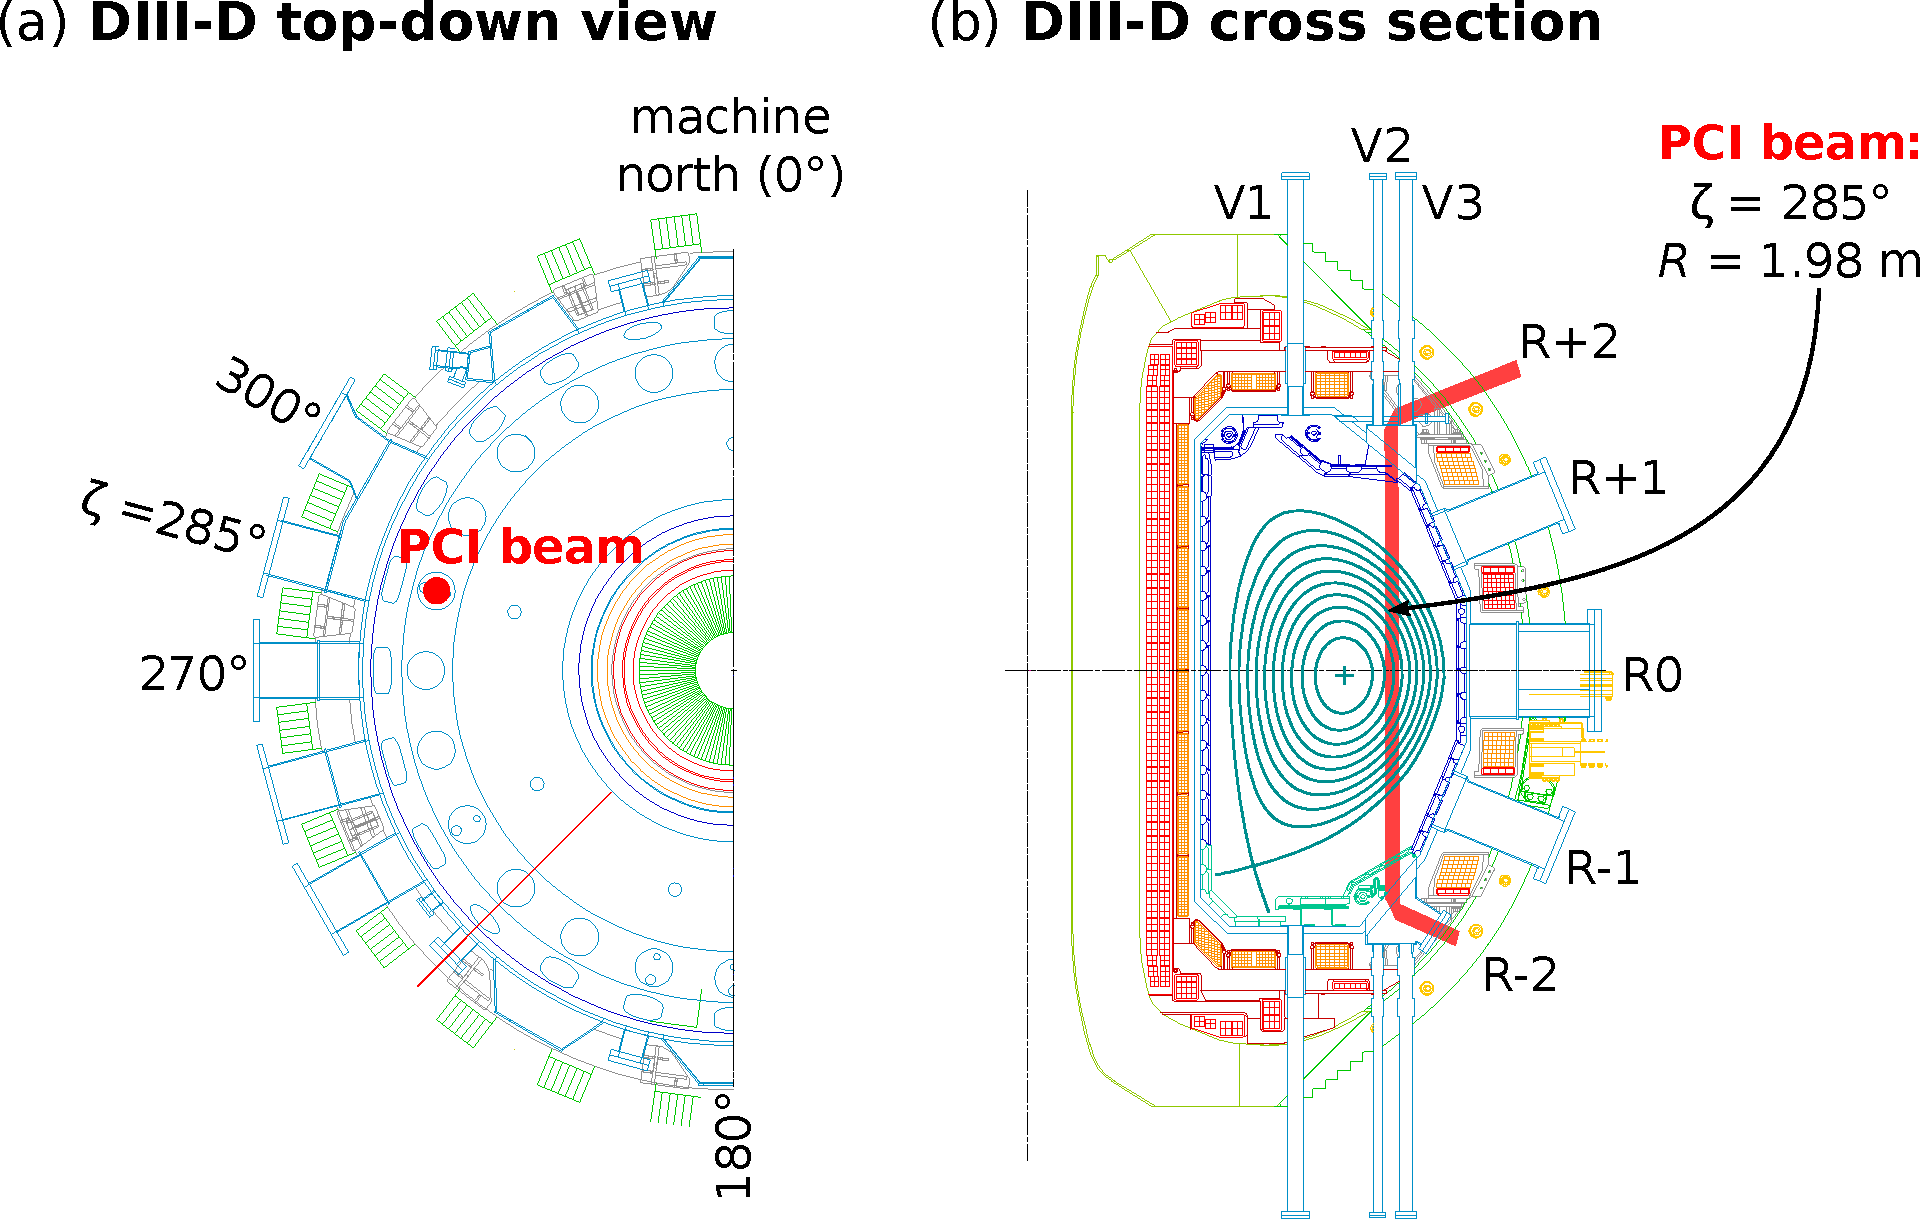
\includegraphics[width = \textwidth]{%
    Chapters/Implementation/figs/d3d_port_locations.pdf}
  \caption[\diiid \space port-labeling conventions and location of PCI]{%
    (a) View of \diiid \space from above,
    indicating the toroidal-labeling convention.
    (b) View of \diiid \space cross section,
    indicating the labeling convention
    for vertical (V) and radial (R) sightlines.
    The PCI beam enters the vessel through the $285^{\circ}$ R+2 port,
    propagates vertically downwards through the plasma
    at a major radius of $R = \SI{1.98}{\meter}$, and
    exits the vessel through the $285^{\circ}$ R-2 port.}
\label{fig:Implementation:d3d_port_locations}
\end{figure}


\section{\diiid's pre-existing PCI system}
The \diiid \space PCI system is
thoroughly described elsewhere~\cite{dorris_rsi09, dorris_phd}, but
the system components of relevance to this work
are briefly summarized below for completeness.


\subsection{System geometry}
The system is currently configured
in the ``Phase II'' geometry~\cite{dorris_rsi09},
with the probe beam propagating vertically downwards
from the $285^{\circ}$ R+2 port to the $285^{\circ}$ R-2 port.
The beam center sits at $R = $ \SI{1.98}{\meter}.
Both the toroidal and radial positions
of the PCI beam are shown in
Fig.~\ref{fig:Implementation:d3d_port_locations}.

The PCI system's vertical beam path constrains
which types of fluctuations it can and cannot detect.
Namely, the PCI-measured power fluctuations
(\ref{eq:InterferometricMethods:PCI_ratio_fluctuating_to_equilibrium_power})
correspond to \emph{line-integrated} electron-density fluctuations, which
are the physical origin of the phase fluctuations $\tilde{\phi}$ in
(\ref{eq:InterferometricMethods:phase_fluctuation}).
Because it is a line-integrated measurement,
only fluctuations propagating perpendicular to the beam path can be detected,
as fluctuations propagating parallel to the beam path
are effectively averaged out of the signal
\graffito{\textcolor{red}{what about $\delta \omega$?}}
(and, at a more fundamental level, fluctuations propagating
parallel to the beam path do \emph{not} spatially scatter the probe beam).
\graffito{\textcolor{red}{citation? Wesson?}}
Now, electrostatic turbulence (e.g.\ ITG, ETG) tends to be field-aligned
such that $k_{\perp} \gg k_{||}$, where
the $\perp$ and $||$ subscripts are used here to indicate
orientations that are perpendicular to and parallel to
the local magnetic field, respectively.
To lowest order, then, electrostatic fluctuations propagate
perpendicular to a tokamak's toroidal field.
PCI's vertical beam path and
the field-aligned constraint of electrostatic turbulence
imply that PCI is predominantly sensitive to fluctuations
with finite major-radial wavenumber $k_R$.
Thus, PCI's 32-element, 1-dimensional detector array
is oriented in the image plane such that
each detector element corresponds to a unique major radius in the plasma.

In some situations, 2-dimensional detector arrays
\cite{sanin_rsi04, tanaka_rsi16} or
spatially filtering ``masks''~\cite{dorris_rsi09, dorris_phd, lin_rsi06}
can be used to localize measurements
by exploiting the spatial variation
in the magnetic field's orientation along the beam path.
These localization techniques typically work best
for high-$k$ measurements.
Note that $k_R$ is related to the
often-theoretically-relevant poloidal wavenumber $k_{\theta}$ via
\begin{equation}
  k_R = k_{\theta} \csc[\alpha(R, z)],
  \label{eq:Implementation:kR_to_ktheta}
\end{equation}
where $\alpha(R, z)$ is the angle
between the beam path and the local flux surface,
as shown schematically in
Fig.~\ref{fig:Implementation:relating_kR_to_ktheta}.
Of course, the fluctuation measurements must be localized,
either via direct measurement
(with 2-dimensional detector arrays or ``masks'')
or via inference from other plasma properties,
before (\ref{eq:Implementation:kR_to_ktheta})
can be inverted to yield $k_{\theta}$
from measured values of $k_R$.

\begin{figure}
  \centering
  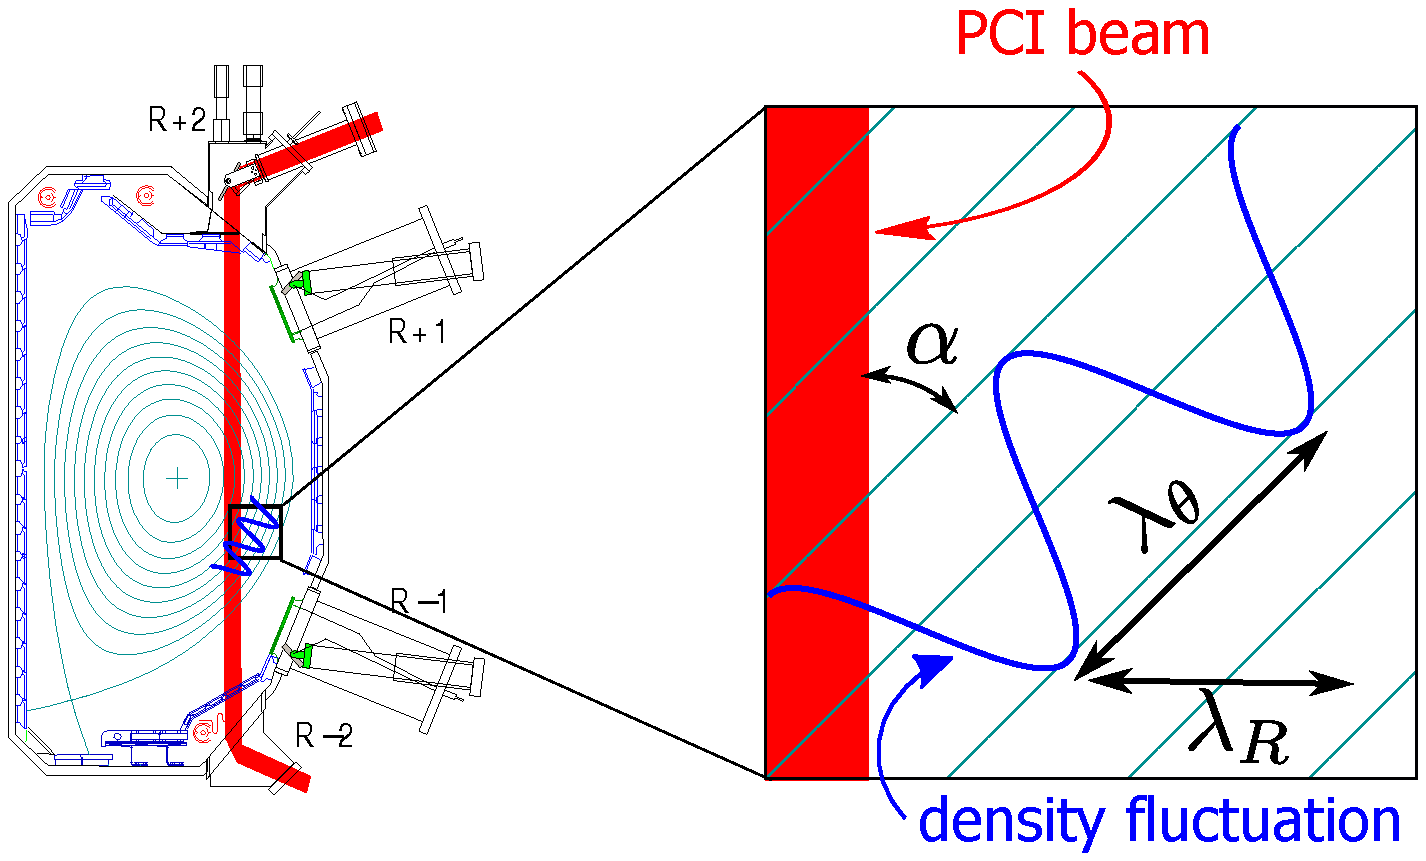
\includegraphics[width = 0.9 \textwidth]{%
    Chapters/Implementation/figs/kR_to_ktheta.pdf}
  \caption[Relating $k_R$ to $k_{\theta}$]{%
    The major-radial wavenumber $k_R = 2 \pi / \lambda_R$ and
    the poloidal wavenumber $k_{\theta} = 2 \pi / \lambda_{\theta}$
    are related via $\alpha(R, z)$, which
    is the angle between PCI's vertical probe beam and
    the local flux surface.}
\label{fig:Implementation:relating_kR_to_ktheta}
\end{figure}


\subsection{Spatial bandwidth}
The system has $k_{\text{min}}^{\text{PCI}} = \SI{1.5}{\per\centi\meter}$.

The 1/e electric field radius of the in-vessel beam is
$w_0 =$ \SI{3.4}{\centi\meter}, and

A pair of fast steering mirrors dynamically centers
the unscattered beam on the phase plate groove,
compensating for vibrations.



\subsection{Temporal bandwidth}


\begin{itemize}
  \item $k$-cutoff
  \item Maintenance
    \begin{itemize}
      \item Replacement of laser
      \item Replacement of feedback detector
      \item Replacement of in-vessel mirrors
    \end{itemize}
\end{itemize}

\section{Interferometer design}
\begin{itemize}
  \item Power sharing between the interferometer arms and PCI
  \item TE-cooled detector
  \item Imaging and $k$-response
  \item Demodulation scheme
\end{itemize}

\section{Interferometer optimization}
\begin{itemize}
  \item LO stability
  \item External clock
\end{itemize}

\section{Sound-wave calibration of combined PCI-interferometer}
\begin{itemize}
  \item Importance of speaker placement
  \item System sensitivity
\end{itemize}


\bibliographystyle{plainurl}
\bibliography{references}
